\documentclass{article}
\usepackage[utf8]{inputenc}
%\usepackage[latin1]{inputenc}
\usepackage[danish]{babel}
%\usepackage[T1]{fontenc}
\usepackage{graphicx}
\graphicspath{{images/}}

\begin{document}
\author{Tor Soya, Alexander Müllertz, og Emil Schytte Bækgaard}
\title{Dokumentation af P.C. Tec Management system}
\date{23. juni 2015}
\maketitle
\newpage
\tableofcontents
\newpage
\section{Logind Sekvens}


På figur \ref{fig:1} ses startsiden. For at logge ind, skal felterne, som er markeret med rødt, oppe i højre side af skærm billedet udfyldes og der skal trykkes på login.
\begin{figure}[ht]
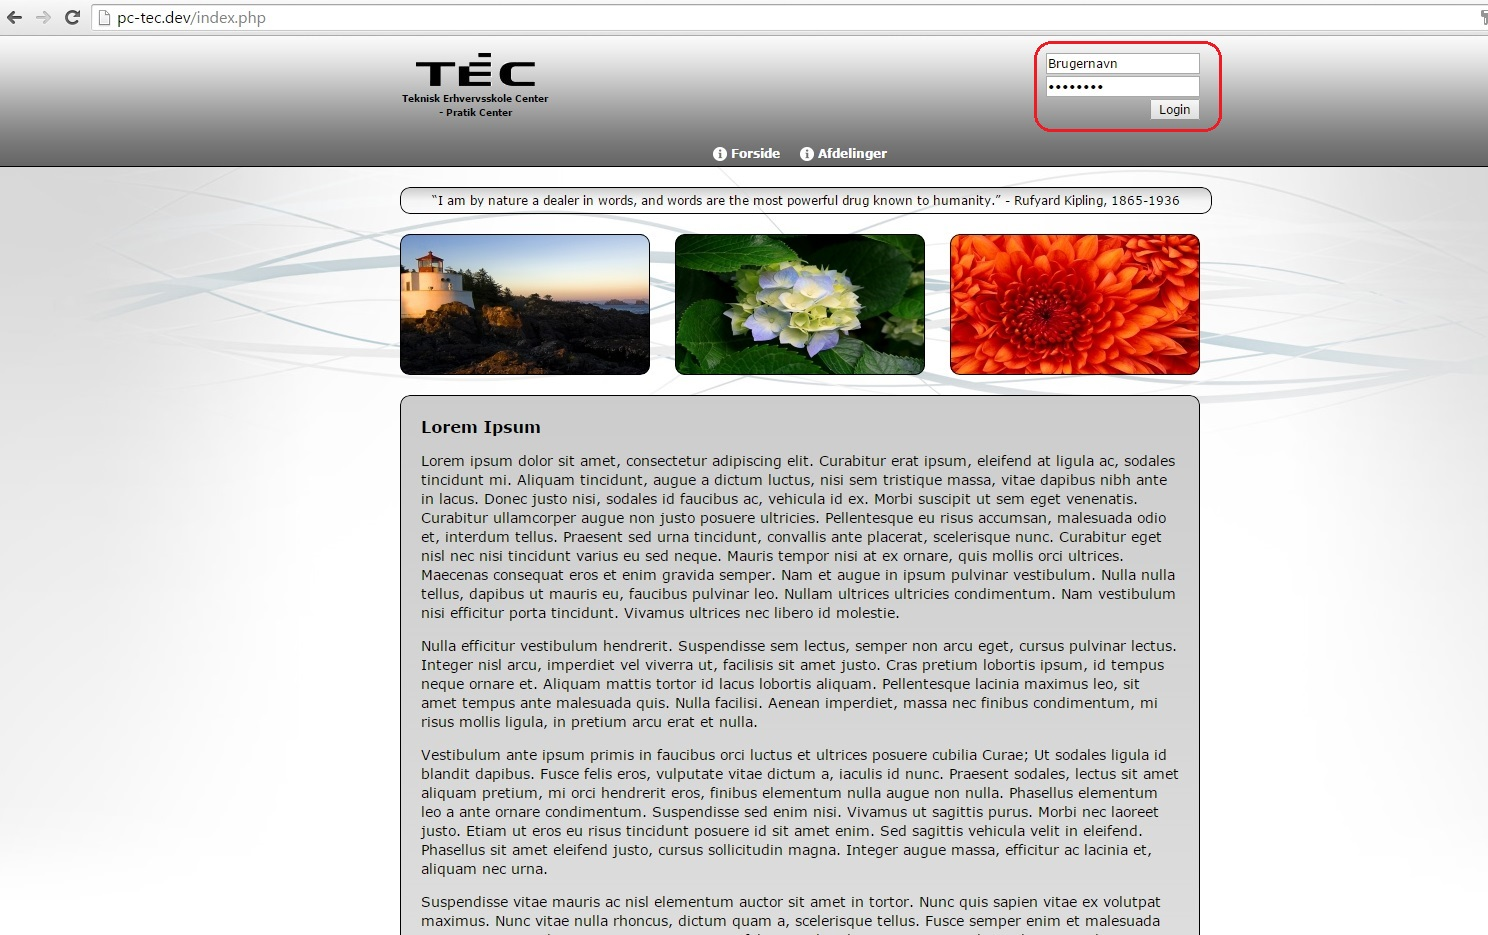
\includegraphics[width=343px]{startside.jpg}
\caption{Startside}
\label{fig:1}
\end{figure}

\section{Brugermenu}
I brugermenuen vises alle de relevante links til at navigere rundt på siden.\\
Menuen indeholder punkterne :
\begin{itemize}
\item Min Profil
\item Projekter
\item Brugere
\item Administration (vises kun for instruktører og værkføre)
\item Log ud
\end{itemize}
Disse punkter vises også i på figur \ref{fig:2}

\begin{figure}[ht]
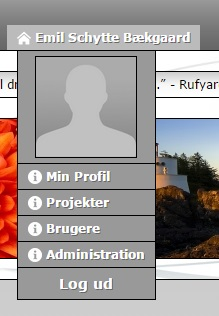
\includegraphics[width=150px]{brugermenu.jpg}
\caption{Brugermenu}
\label{fig:2}
\end{figure}

\newpage
\section{Min Profil}
Under min profil vil der blive vist generelle oplysninger, herunder hvilken uddannelse brugeren er på, hvilken funktion brugeren har, hvilke kompetencer brugeren har og hvor mange dage brugeren har tilbage før brugeren er færdiguddannet. \\
Der vil også på denne side stå hvilke projekter brugeren er tilknyttet, både afsluttet og igangværende projekter.\\
Brugeren vil her ved at trykke på projektnavnene, komme ind på en side hvor projektets detaljer står uddybet. Siden "Min Profil" vises i figur \ref{fig:3}

\begin{figure}[ht]
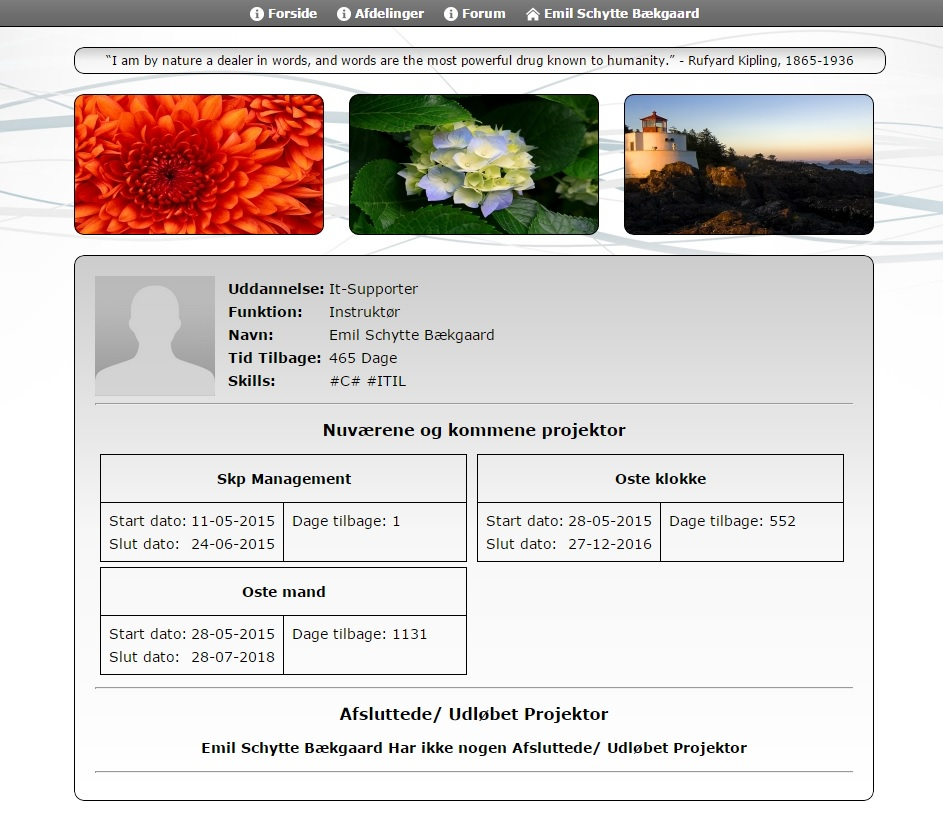
\includegraphics[width=343px]{minprofil.jpg}
\caption{Min Profil}
\label{fig:3}
\end{figure}
 \newpage
\section{Projekter}
Projektre er en stor del af dette system. Meningen er at instruktører og elever får et bedre overblik over hvilke aktiviteter der er igang og hvilke aktiviteter eleverne kan komme i gang med. Menupunktet "Projekter" indeholder følgende underpunkter:
\begin{itemize}
\item Projekt Oversigt
\item Opret Ny Projekt Skabelon
\item Projekt Skabeloner
\end{itemize}
\newpage
\subsection*{Projekt Oversigt}
Viser en liste over de projekter som er aktive i P.C.B. Igen kan brugeren trykke på projektnavnene og se detaljerne for de enkelte projekter. Se evt. Figur \ref{fig:4} 
\begin{figure}[ht]
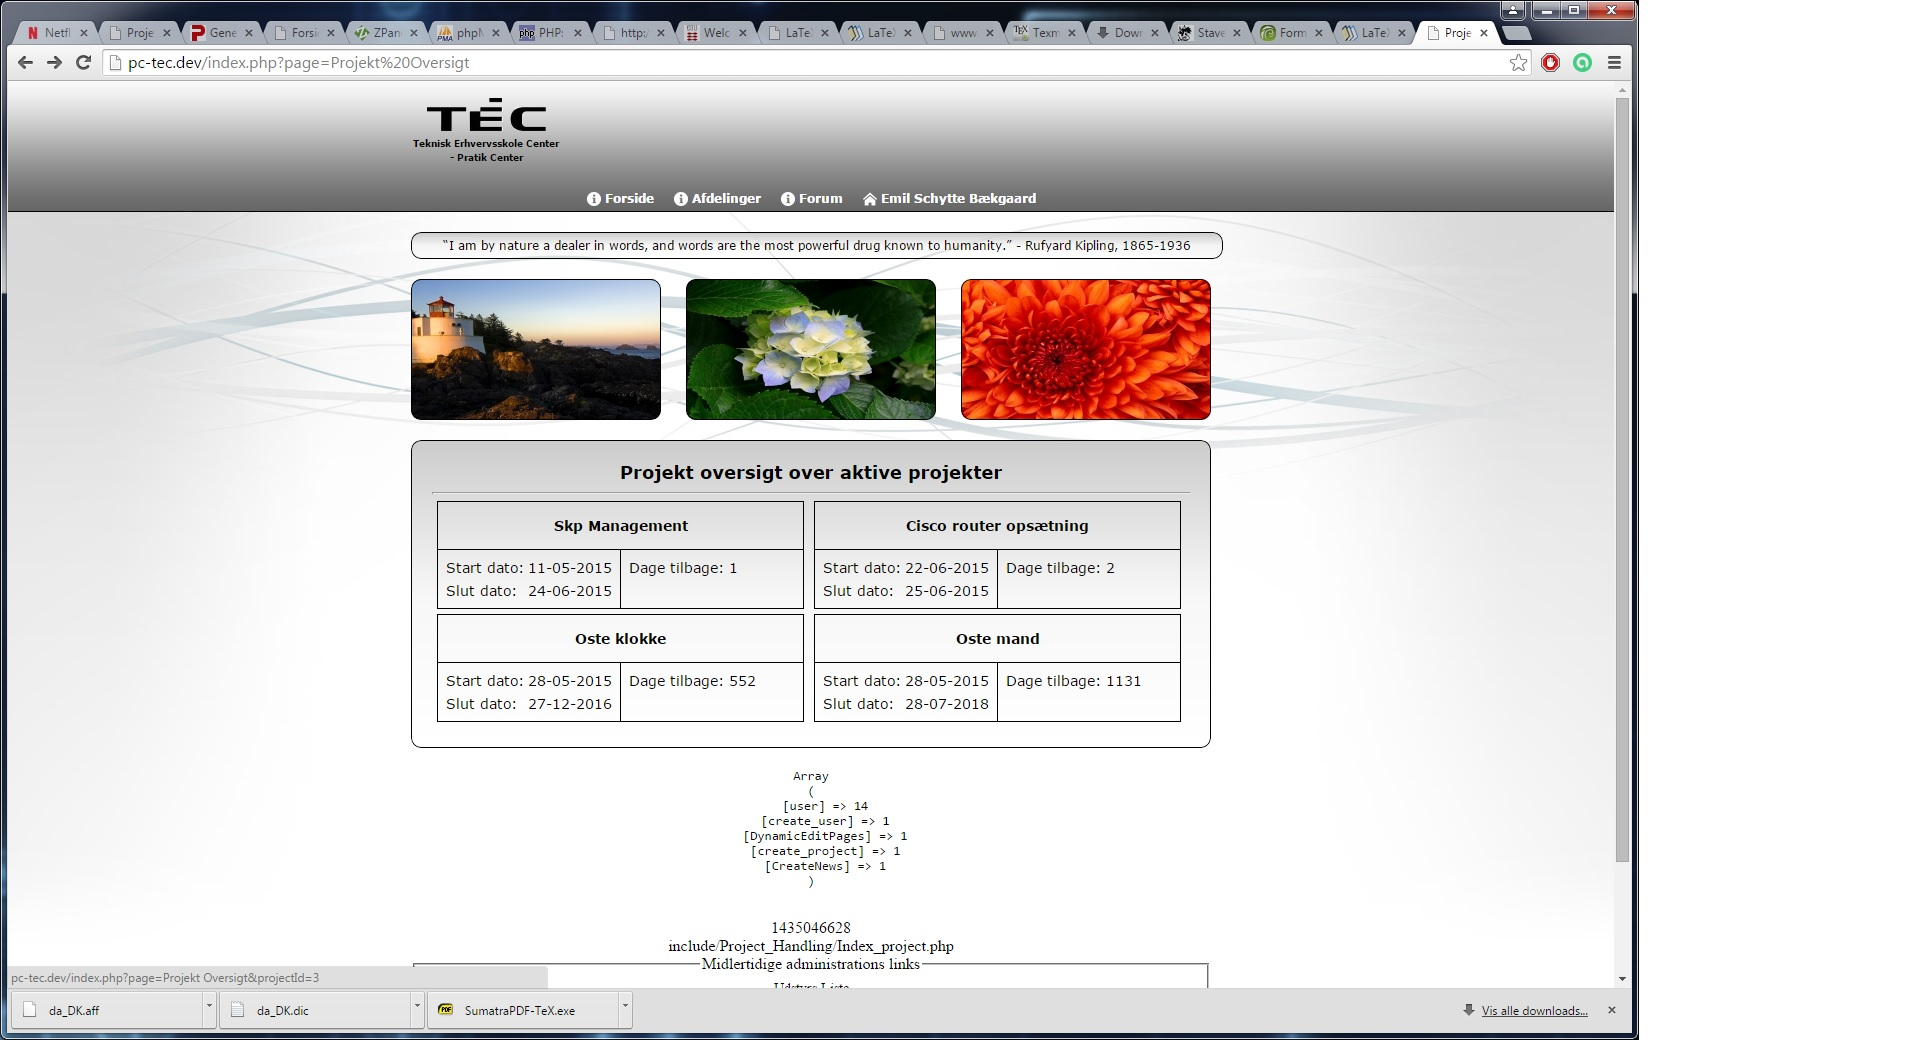
\includegraphics[width=343px]{aktiveprojekter.jpg}
\caption{Liste over aktive projekter}
\label{fig:4}
\end{figure}
\newpage

\subsection*{Opret Ny Projekt Skabelon}
Dette punkt er kun for instruktører. Det er her et projekt starter med at oprette en skabelon som indeholder et navn, en beskrivelse, en kategori, og et link til en evt. kravsspecifikation eller lig. se evt. Figur \ref{fig:5}
\begin{figure}[ht]
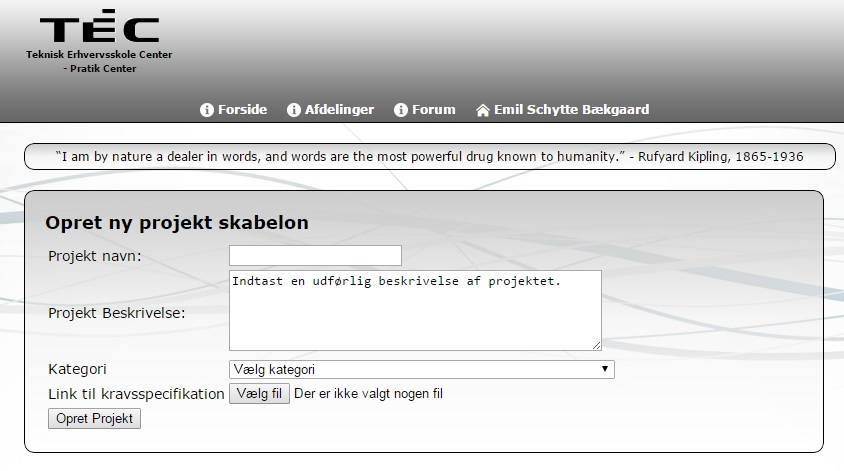
\includegraphics[width=343px]{nyprotemp.jpg}
\caption{Opret projektskabelon}
\label{fig:5}
\end{figure}
\newpage
\subsection*{Projektskabeloner}
Under dette menu punkt bliver en liste af projektskabeloner vist til brugeren. Ved at trykke på et af navnene på projektskabelonerne bliver en side vist hvorfra projektskabelonen kan aktiveres til et aktivt projekt. Se evt. Figur \ref{fig:6}
\begin{figure}[ht]
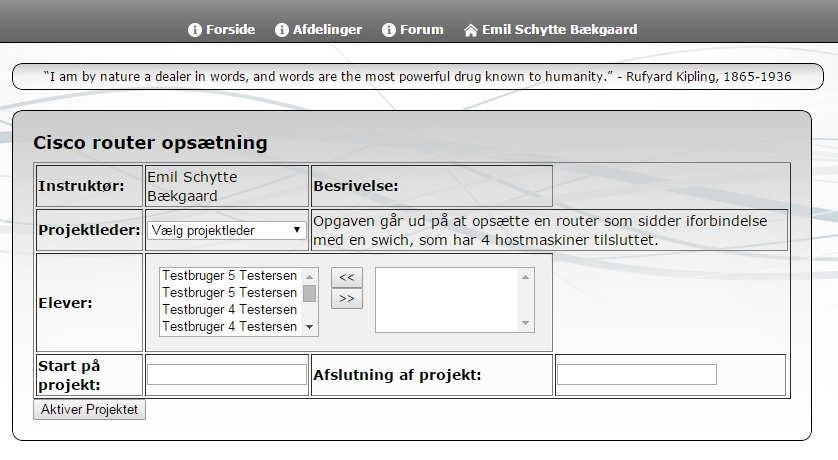
\includegraphics[width=343px]{aktiveverProjekt.jpg}
\caption{Aktiver projektskabelon}
\label{fig:6}
\end{figure}
\newpage
\section{Bruger administration}
\begin{figure}[ht]
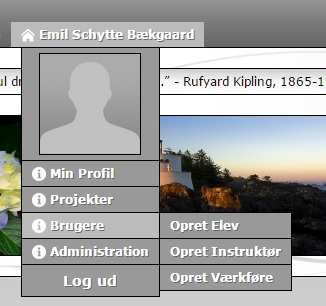
\includegraphics[width=150px]{brugerpunkt.jpg}
\caption{Brugermenu Brugere}
\label{fig:7}
\end{figure}

Punktet Brugere vises kun for instruktører, her inde sker alt administration ang. brugere. Her kan brugeren oprette nye brugere:
\begin{itemize}
\item Opret Elev
\item Opret Instruktør
\item Opret Værkføre
\end{itemize}
\subsection*{Opret Elev}
Under Opret Elev, kan brugeren oprette nye brugere med rollen Elev. som vist i Figur \ref{fig:8}
\begin{figure}[ht]
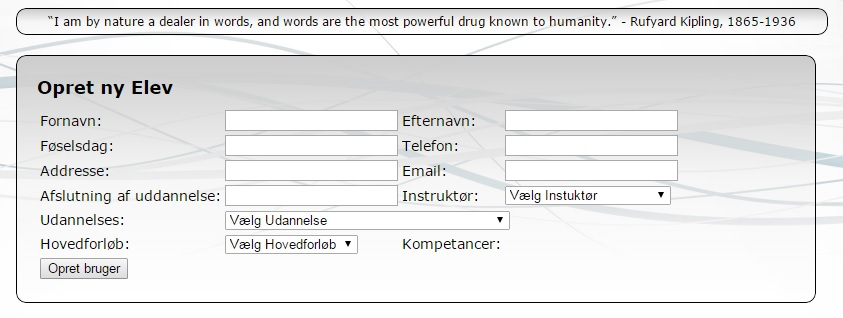
\includegraphics[width=343px]{opretelev.jpg}
\caption{Opret ny elev}
\label{fig:8}
\end{figure}
\newpage
\subsection*{Opret Instruktør}
Her er brugeren i stand til at oprette nye brugere af typen Instruktør, som vist i Figur \ref{fig:9}
\begin{figure}[ht]
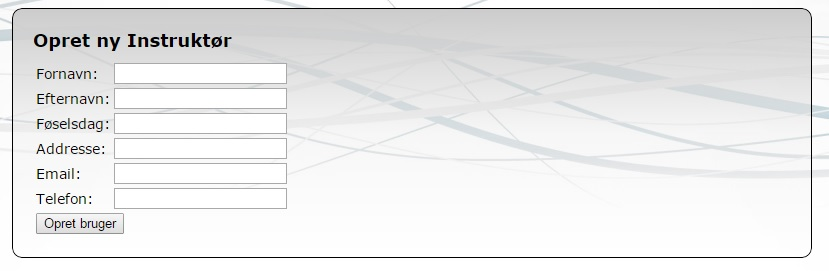
\includegraphics[width=343px]{inst.jpg}
\caption{Opret ny elev}
\label{fig:9}
\end{figure}

\subsection*{Opret Værkføre}
For at oprette værkføre skal instruktøren ind under dette punkt i brugermenuen under "Bruger" og derefter under "Opret Værkføre". Det er samme form som vist i Figur \ref{fig:8} bare med overskriften: "Opret ny Værkføre"
\newpage
\section{Administration}
Denne del omhandler punktet "Administration" under brugermenuen. Her vil brugeren kunne oprette nyheder samt at kunne ændre i den menu som hedder "Afdelinger".
\subsection*{Nyheds Administration}
Brugeren af typen instruktør og værkføre, vil her kunne oprette/rette/slette nyheder, som vist på figur \ref{fig:10}
\begin{figure}[ht]
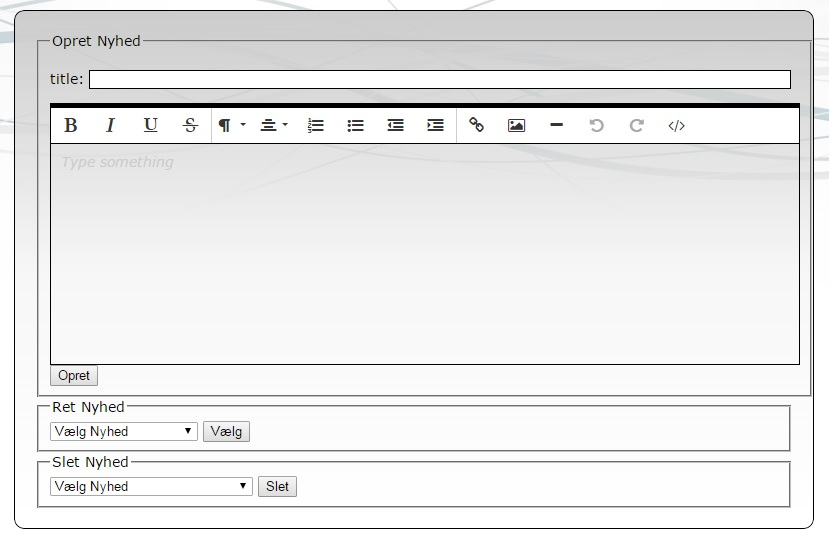
\includegraphics[width=343px]{nyhedadmin.jpg}
\caption{Administration af nyhedder}
\label{fig:10}
\end{figure}
\newpage
\subsection*{Menu Administration}
Instruktører og værkfører vil her kunne ændre menuen "afdelinger" se Figur \ref{fig:11}
\begin{figure}[ht]
\begin{center}
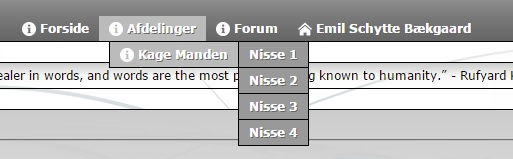
\includegraphics[width=150px]{navMenu.jpg}
\end{center}

\caption{Navigations Menu}

\label{fig:11}
\end{figure}
Dette er en menu der er tiltænkt til de sider som hver afdeling kan have, med en beskrivelse af afdelingen, med billeder osv. 
Et eksempel med fyldtekst kan ses på Figur \ref{fig:12}
\begin{figure}[ht]
\begin{center}
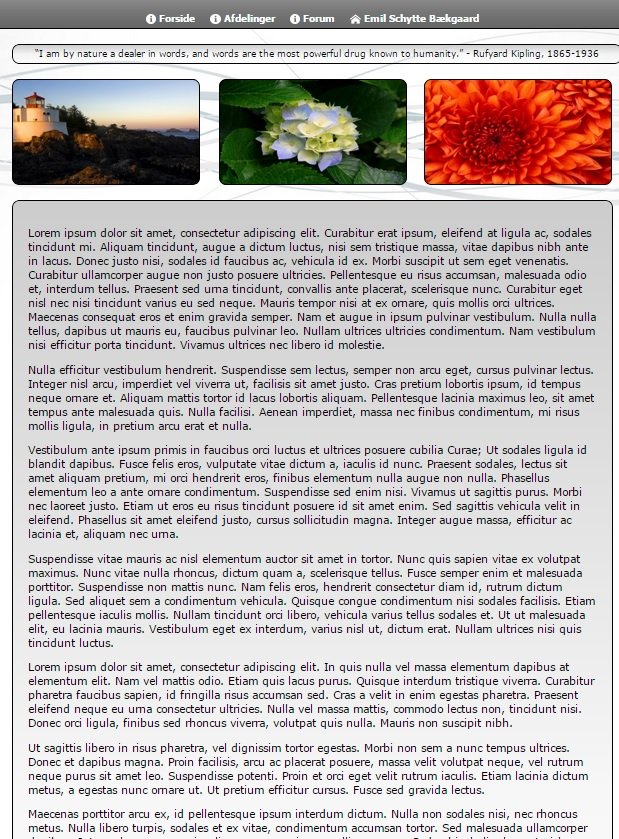
\includegraphics[width=0.5\textwidth]{afdelingsside.jpg}
\end{center}

\caption{Eksempel på en afdelingsside}
\label{fig:12}
\end{figure}

\end{document}